\documentclass[usenatbib]{mn2e}
\usepackage[pdftex]{graphicx}
\newcommand{\be}{\begin{equation}}
\newcommand{\ee}{\end{equation}}
\newcommand{\bea}{\begin{eqnarray}}
\newcommand{\eea}{\end{eqnarray}}
\newcommand{\bc}{\begin{center}}
\newcommand{\ec}{\end{center}}
\newcommand{\ol}[1]{ {\overline{#1}}}
\newcommand{\lu}{\,h^{-1}{\rm kpc}}
\renewcommand{\vec}[1]{ {\bmath #1} } 
\newcommand{\e}{{\rm e}}
\newcommand{\dd}{{\rm d}}
\newcommand{\ap}[1]{\textcolor{magenta}{#1}}
\def\gsim{ \lower .75ex \hbox{$\sim$} \llap{\raise .27ex \hbox{$>$}} }
\def\lsim{ \lower .75ex \hbox{$\sim$} \llap{\raise .27ex \hbox{$<$}} }

% Individual page for figures
\usepackage{afterpage}

% Fancy merger rate symbol:
\usepackage{amssymb}
\usepackage{amsmath}
\usepackage[amssymb]{SIunits} 

% Make font much more compact
\usepackage{times}

% Compact lists (compactitem):
\usepackage{paralist}

% References highlighted in blue (include "draft" option for troubleshooting)
\usepackage[bookmarks,bookmarksnumbered,colorlinks=true,citecolor=blue,linkcolor=blue]{hyperref}
\usepackage{color}

% Line break inside table cell
\usepackage{pbox}

% Vertical spaces in table
\usepackage{booktabs}

% Tables with notes, etc.
\usepackage[flushleft]{threeparttable}

% Blocks of comments
\usepackage{comment} 

% Color highlighting
\definecolor{darkgreen}{rgb}{0.0, 0.5, 0.0}
\newcommand{\highlight}[1]{{\color{darkgreen} #1}}

% Custom commands, to be used inside math environment:
\newcommand{\Msun}{{\rm M_{\odot}}}

\setlength{\topmargin}{-1.2cm}

\renewcommand{\thefootnote}{\fnsymbol{footnote}}



\usepackage{booktabs}
\usepackage{hhline}
\usepackage{breqn}
\usepackage{standalone}
\usepackage{dcolumn}
	\newcolumntype{d}[1]{D{.}{.}{#1}}
\usepackage{tabularx}
\usepackage{booktabs}
\usepackage{microtype}
\usepackage{algpseudocode}
\usepackage[]{algorithm2e}
\usepackage[update,prepend]{epstopdf}
\epstopdfsetup{outdir=./figures/finalized/}
\graphicspath{{./figures/finalized}{figures/drafts/}}

\newcommand{\mc}[1]{\multicolumn{1}{c}{#1}} % handy shortcut macro
%-----------------------------------------------------------------------
\def\Hmat{\mathbf{\it H}}
\def\apjl{ApJL }
\def\aj{AJ }
\def\apj{ApJ }
\def\pasp{PASP }
\def\spie{SPIE }
\def\apjs{ApJS }
\def\araa{ARAA }
\def\aap{A\&A }
\def\nat{Nature }
\def\mnras{MNRAS }
\def\mnrasl{MNRASL }
\providecommand{\eprint}[1]{\href{http://arxiv.org/abs/#1}{#1}}
\providecommand{\adsurl}[1]{\href{#1}{ADS}}
\providecommand{\ISBN}[1]{\href{http://cosmologist.info/ISBN/#1}{ISBN: #1}} 
%-----------------------------------------------------------------------
\title[Galaxy-dark matter offsets in galaxy clusters and groups of the
Illustris simulation]
{Galaxy-dark matter offsets in galaxy clusters and groups of the
Illustris simulation}
\author[Karen Y. Ng et al.]{Karen Y. Ng,$^{1}$
	Annalisa P. Pillepich,$^{2}$ 
	William A. Dawson,$^{3}$ 
	D. Wittman,$^{1}$
	\newauthor Lars Hernquist,$^{2}$
	etc. [order TBD]
}
\begin{document}
\date{arXiv} \pagerange{\pageref{firstpage}--\pageref{lastpage}}
\pubyear{2015} \maketitle\label{firstpage}
\begin{abstract} 
	Galaxy clusters, which mainly compose of dark matter (DM), 
	can be rare test beds for the particle properties of DM.
	However, the continuous merger and accretion events of clusters also
	complicate the modeling of galaxy clusters.
	With uncertainties coming from various modeling choices and observational constraints, 
	we need to carefully account for the
	uncertainties for us to give meaningful quantitative constraints from 
	the studies of galaxy clusters. In this paper, 
	we test various summary statistics of the different components
	of galaxy clusters by applying them to data from a cosmological simulation,
	the Illustris simulation. 
	We examine the uncertainties of the different one-point statistics that
	are intermediate quantities for computing the spatial offsets between
	the member galaxies and the dark matter components. 
\end{abstract}

\begin{keywords}
	galaxy clusters, dark matter, statistics 
\end{keywords}

\section{INTRODUCTION} 
Galaxies that belong to a galaxy cluster or group represents the overdensities
of the underlying dark matter (DM) distribution. 
% Why we want to compare galaxies with the DM distribution? 
There have been many literature that tried to compare the galaxies and the DM
distribution. 


% What are the observational methods for summarizing dark matter distribution?
Weak and strong lensing for finding out the dark matter distribution. 
While 
Common to all the methods are the estimation of the density peaks. 
Convergence map.  


% What are the methods for summarizing the galaxy distribution?
There are many reasonable models for summarizing the overall spatial
distribution of cluster components. Each method has different uncertainties.
They fall under several categories, 1) mixture models, 2) basis function
expansions, such as wavelet methods 
 and 3) non-parametric estimations such as a kernel density estimation. 
 Not only do the performance of the first two methods depend heavily on model parameters, 
the data fit also depend quite strongly on the underlying mixture model /
wavelet basis. Often times, the most common mixture models and wavelet bases 
carry symmetry assumptions that may not be valid for galaxy clusters. 
This is because galaxy clusters have substructures over a wide range of length
scales, from galaxy scales of hundreds of pc to fraction of a Mpc. 
The symmetry assumption will bias the estimate of the point estimate that we
are after for non-symmetric clusters.

We quantify the bias and uncertainty associated with the one-point summary
statistic for summarizing the physical state of a galaxy cluster. 
Commonly used one-point statistic of galaxy clusters include:
1) papers reported using centroids but did not state what centroid that they
used 
2) papers used center of mass 
3) papers that used peaks  
% What are the reported offsets?
Uncertainties affect the conclusion for the computation the hypothesis test / parameter
estimation
Previous work on quantifying galaxy-DM offsets included  
What centroids they have used

Physical motivation for using the galaxy density peak 

In this paper, we 
1) extract realistic observables from the Illustris simulation for
comparison with observations, 2) identify practical, objective one-point statistic for 
summarizing the member galaxy population of a galaxy cluster, 3)	
give estimates for the offsets between the summary statistics of the galaxy  
population and the DM population. We call this offset as 
\begin{equation}
	\Delta s \equiv |\vec{s}_{gal} - \vec{s}_{DM}|,
\end{equation}
where $\bf{s}_{gal}$ and $\bf{s}_{DM}$ are the two dimensional (2D) spatial
locations of the summary statistic of the galaxy population, and the density
peak of DM respectively. 
Finally, we provide the distribution and investigrate origin of $\Delta s$. 

% how are things called in the Illustris simulation?


In section \ref{sec:illustris_sim},
we will describe the physical properties of the products of the Illustris
simulation, and the selection criteria that we have employed to ensure that the
quantities that we examine resemble observables but without noise and
systematics from observations. Then in section ? we will describe the methods for computing various 
one-point statistics of the spatial distribution of galaxies how we prepare our dark
matter spatial data to resemble convergence maps. We will show the comparison
of the different summary statistics in section before we show the main results
in section . 

\section{The Illustris simulation data} 
\label{sec:illustris_sim}
The data that we use: The Illustris simulation 
one of the most detailed cosmological simulations of our universe. 
Under the assumed Lambda Cold Dark Matter cosmology, it is unclear 
that how large the offset $\Delta \vec{s}$ should be. 


Our analyses make use of the same cosmology as the Illustris simulation.
The highest resolution Illustris-1 simulation. 
With a snapshot at $z=0$. 
Two sets of halo finder - one is for halo sized stuff 
the other one for particles Subfind 
Terminology 
halos - what we refer to cluster sized halos identified by RockStar  / Subfind 

subhalos - galaxy sized  
observation bands $u, g, r, i, z$



\begin{figure*}
	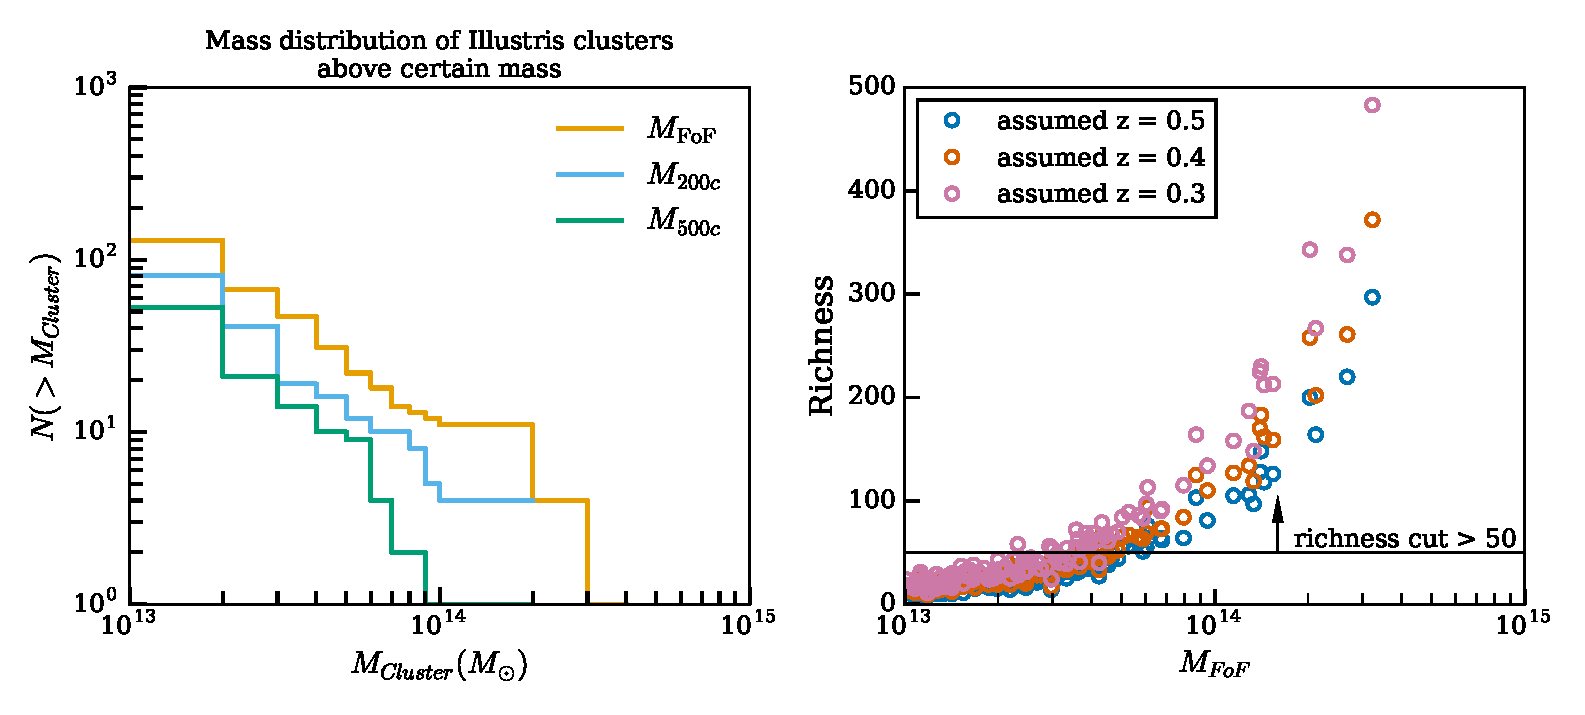
\includegraphics[width=\linewidth]{./figures/finalized/clusterMassDist.eps}
	\caption{ {\bf Left figure:} Mass distribution of the group / cluster sized DM halos
		for different halo selection schemes. Mass estimates obtained by the
		Friends-of-Friends RockStar algorithm are labeled as  M$_{\text{FoF}}$.
		Masses centered on the most bound particle within a radius those the 
		average density is 200 or 500 times the critical density of the universe are 
		labeled as M$_{200c}$ and M$_{500c}$ respectively. 
		Discrepancies between the different
		measures of mass of the clusters indicate the presence of spatially
		separated substructures for the clusters (See Fig ? ). {\bf Right figure:} Mass-richness
		relationship of galaxy clusters and groups with $M_{FoF} > 10^{13} M_{}$ . We require clusters to have more than 50 member galaxies that
	are above observation limit, i.e. apparent $i \leq 24$ when we assume a cosmological redshift
of $z=0.4$, as shown by the richness cut. \label{fig:mass_richness}}

\end{figure*}

Finally, for our final results, we only make use of galaxy clusters / groups 
that have at least 50 member galaxies after this magnitude cut. This is because
of the relatively large statistical uncertainty from small number summary
statistics. 

\subsection{Selection of the field of view}
\label{sec:FOV}
As a default output from the Illustris simulation, subhalos and particles of
each galaxy cluster and group are identified by the Rockstar halo finder
(CITATION). We make use of the member particle / subhalo identification as our
default volume selection scheme for each cluster / group.
We understand that this choice of volume selection can be more ideal than
observational conditions. We make use of this volume selection scheme
for baseline comparisons. 

Furthermore, assuming a conservative line-of-sight (los) distance 
, i.e. cosmological redshift, of $z = 0.4$, 
the projected extent for most of the Illustris galaxy clusters and groups, 
fits inside the field of view of telescopes, such as the Subaru Suprime Camera,
which covers a physical area of $\sim 9$ Mpc $\times 7$ Mpc. 

\subsubsection{Spatial Projections}
The center findings are all based on two-dimensional (2D) matter projections.
In order represent the projection uncertainty, we sample the projections evenly
by using HealPy (CITE), which is a Python wrapper for HealPix (CITE).


\begin{table*}
\begin{center}
\begin{minipage}{180mm} 
	\caption{ Selection criteria for stellar subhalos (member galaxies) for each
		cluster / group 
\label{tab:member_galaxy_selections}} 
	\begin{tabular}{@{}lcccc@{}}
\hline 
Data &  Selection strategy  & Sensitivity & Relevant section  \\ \hline
Field of view (FOV) & RockStar halo finder& comparable to FOV of the Subaru
Suprime camera &   \\ 
Observed filter & $i$-band & consistent over the redder $r, i, z$ bands &   \\ 
Richness of member galaxies & $i \leq 24$ and $z = 0.4$  & sensitive to
the assumed cosmological redshift of cluster and &    \\ 
& & the assumed limiting magnitude of telescope &   \\
Two-dimensional projections & even HealPix samples over half a sphere &
discussed as results  & \\  
\hline
\end{tabular} 
\label{tab:selection_criteria} 
\footnotesize{
}
\end{minipage}
\end{center} 
\end{table*}


\begin{table*}
\begin{center}
\begin{minipage}{180mm} 
	\caption{Comparison between various methods for estimating one-point
		statistics of the galaxies of a cluster 
\label{tab:centroid_comparison}} 
	\begin{tabular}{@{}lccccc@{}}
\hline 
Method &  One-point statistic & Sensitivity to biases & Uncertainty  & Relevant
section & Comment  \\ \hline
Centroid & 2D spatial averages & High & Low & \\
Shrinking aperture & proxy for density peak & High sensitivity to substructures & Medium
& \\
Peak finding from KDE & density peak & Lower sensitivity to substructures &
Higher & \\
Brightest cluster galaxy & & Sensitive to foreground contaminants & \\ 
Most bound particle & bottom of gravitational potential well &  & 
&  \\
\hline
\end{tabular} 
\label{tab:summary_stat_info} 
\footnotesize{
}
\end{minipage}
\end{center} 
\end{table*}
\subsubsection{Galaxy weights}
\label{subsubsec:galaxy_weights}
Not all galaxies are created equal, so they should not be considered with equal
importance. Galaxies reside in host halos with different masses and 
contain different stellar masses. The brightness of galaxies in a cluster are 
also affected by the cluster environments.
For example the star formation rates of cluster galaxies are known to be 
suppressed by the high concentration of intracluster medium. (CITE)
One of the most common weighting schemes employed for galaxy data is to weight
by the luminosity in a particular band.
We examined 

\subsubsection{Cluster properties}
\label{subsubsec:cluster_properties}

\subsection{Relaxedness of the clusters}
On the relaxedness of the clusters.
We provide several definitions of non-relaxedness to characterize whether
the clusters underwent any recent merger activities. 
These definitions of non-relaxedness include.
\begin{itemize}
	\item ratio of mass outside the dominant dark matter halo over the total mass
		of the galaxy cluster 
	\item distance between the most bound particle from the center of mass as a
		function of $R_{200c}$.
\end{itemize}

% \begin{figure*}
% 	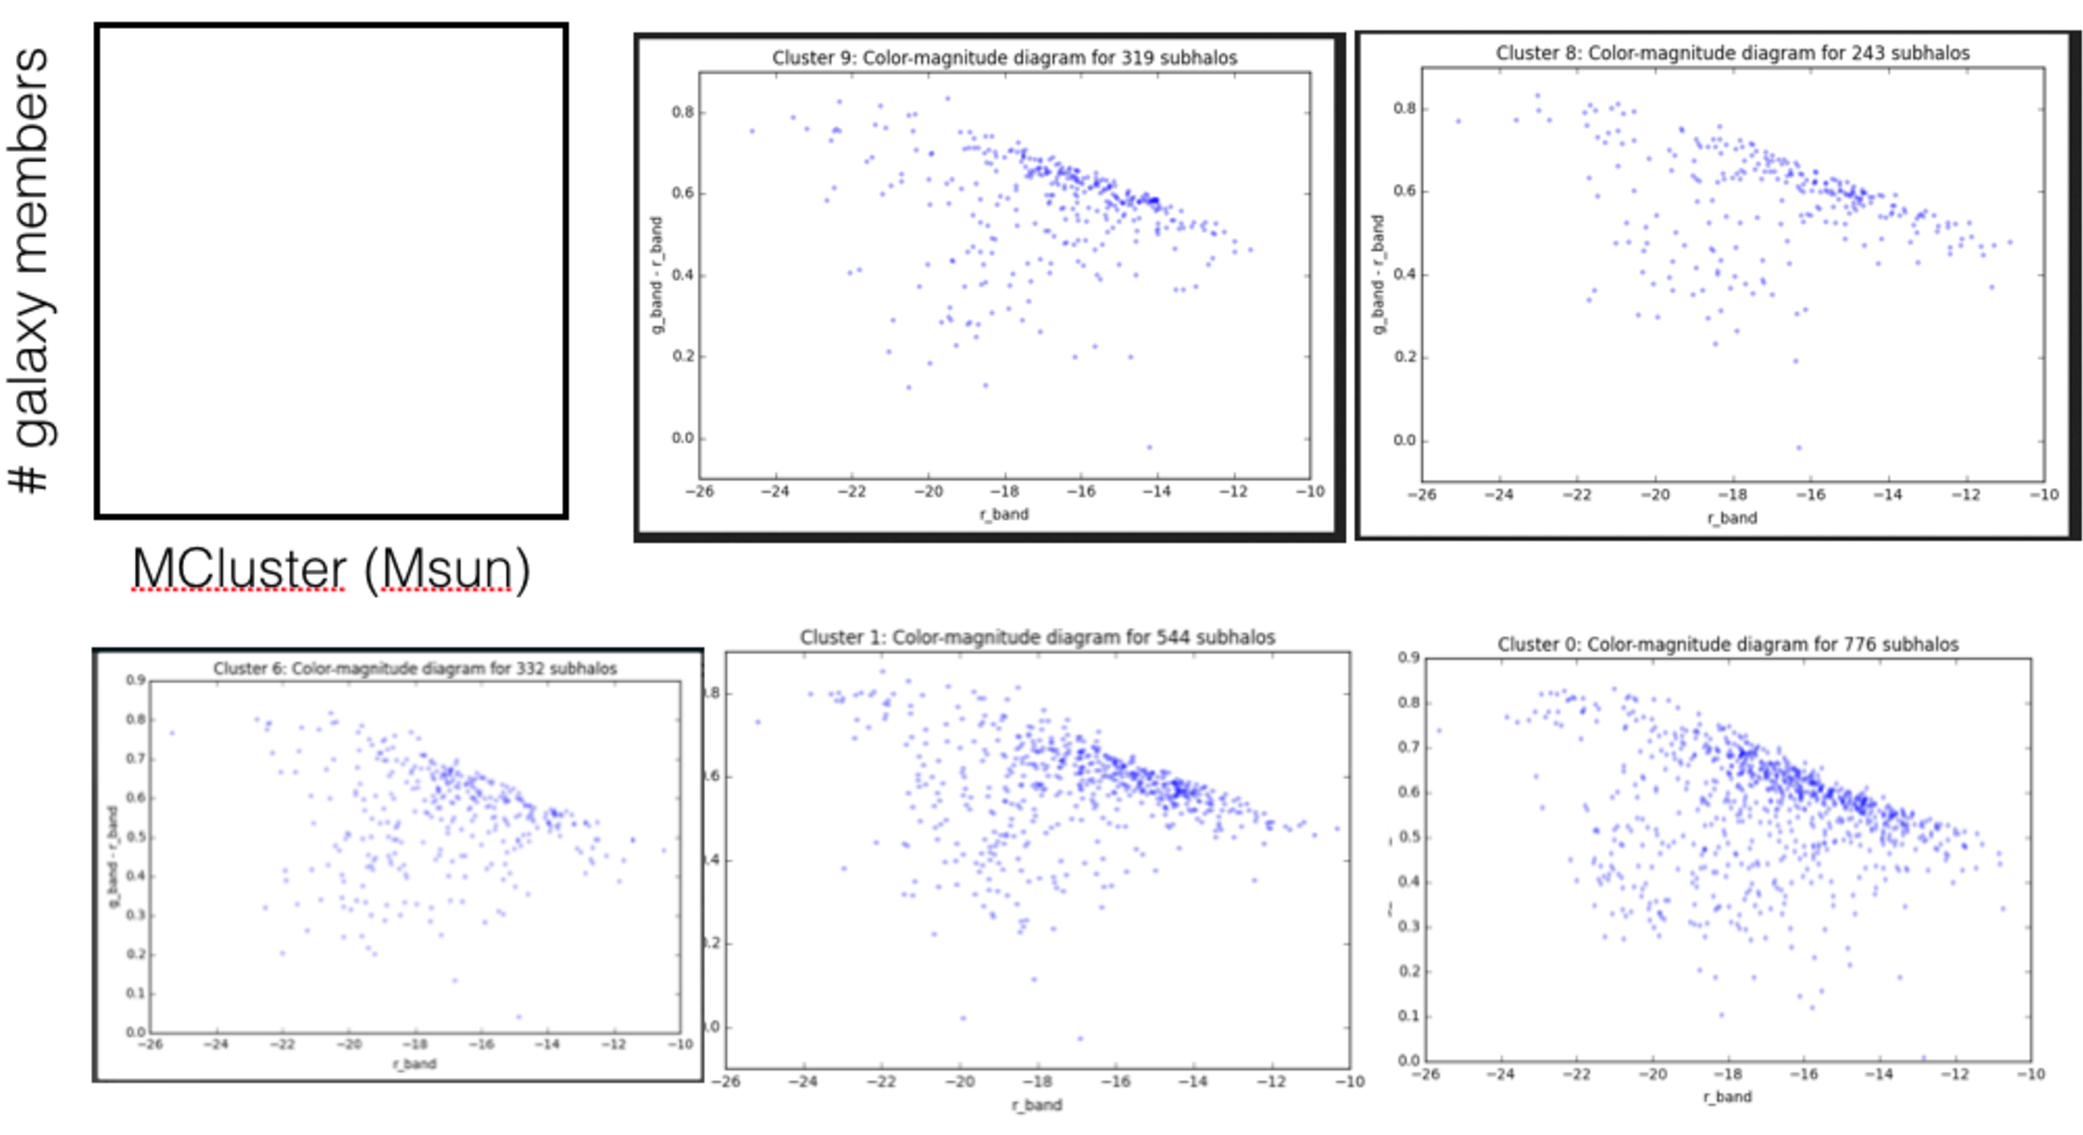
\includegraphics[width=.95\linewidth]{figures/ph_fig_richnessAndColorMagnitudes.pdf}
% 	\caption{
% 		\label{fig:config}}
% \end{figure*}

\section{Methods for summarizing the spatial distribution of ??}

Well known tradeoff Bias-variance tradeoff



Goal: to identify the ``center'' of the light distribution. Here the adopted tracers for the light distribution are the member galaxies of the cluster and groups.

We compare four ways to identify the light/galaxy centers:
\begin{enumerate}
\item Centroids
\item KDE + peak finder
\item Shrinking aperture method
\item Brightest cluster galaxy (BCG)

\end{enumerate}

\subsubsection{Centroids or center of mass}
\label{Unweighted}
We follow the usual definition of spatial centroid as 
\begin{equation}
	\bar{\bf x} = \frac{1}{n} \sum_i \vec{x}_i. 
\end{equation}
While the weighted centroids are just: 
\begin{equation}
	\bar{\bf x}_w = \frac{\sum_i w_i \vec{x}_i}{\sum_i w_i},
\end{equation}
for each spatial dimension and the weights $w_i$ for the $i$-th galaxy
is described in section.
Centroids can be biased 1) by subcomponents from merging activities yet do
not provide explicit evidence for ongoing merger or accretion, 2) by the 
field of view.

\subsubsection{Cross-validated Kernel Density Estimation (KDE) and the peak finder} 
We employed a KDE algorithm to infer a smooth density distribution of the
galaxies.
It is known that the choice of the functional form of the smoothing kernel does
not dominate the density estimate $\hat{f}$ as long as the chosen kernel is
smooth (CITE). Instead we focus our effort to use cross-validation to obtain the optimal 2D smoothing
bandwidth matrix for each cluster ($\Hmat$) for our 2D Gaussian kernel. 
\begin{align}
	\hat{f}(X; \Hmat) &= \frac{1}{n} \frac{1}{(2\pi)^{d/2}|\Hmat|^{1/2}}
	\sum_{i=1}^n \exp((X-{\bf x}_i)^T H^{-1} (X-{\bf x}_i)),
\end{align}
where the dimensionality is $d=2$ for our projected quantities,
$X$ represents the uniform grid points for evaluation, and 
$\bf{x}_i$ contains the spatial coordinates for each of the identified member galaxies 
that survived our brightness cut.

Specifically, we made use of the KDE function in
the statistical package ks (Duong) in the R statistical computing environment 
(R Core Team 2014).
Cross validation eliminates free parameters in the KDE and minimizes
the asymptotic mean-integrated squared error (AMISE) for a best fit to the
data.

After obtaining the KDE estimate, we employed a finite differencing algorithm
to find the local maxima. We sorted the local maxima according to the KDE
density at the maxima locations and identified the dominant peak. 

Spatial location and the density of the subdominant peaks are also stored.
We investigated if the presence of subdominant peaks are correlated with
$\Delta s$. 





\subsubsection{Shrinking aperture}
Another popular method among astronomers for finding the peak of a spatial
distribution include what we call a shrinking aperture method.
We test if the shrinking aperture method is able to reliably recover the highest peak.
This method is dependent on the initial diameter and the initial center location of the aperture.
This method does not evaluate if the cluster is consist of
several subcomponents so the peak estimate can be easily biased by
substructures. Furthermore, the convergence rate for this iterative algorithm is not
analytical and is dependent on the data. We present the
convergence criteria for reference. 
We note that the exact implementation may result in different performances.
\begin{algorithm}
	\caption{Shrinking aperture algorithm}
	\KwData{subhalo that satisfy cuts as a galaxy}
	 \hrulefill

	initial_center = mean(data\_array)\\
 	dist\_array = euclidean_dist(initial_center, data_array)\\
 	apert = get\_90th\_percentile(dist\_array)\\ 
	\While{ (newCenterDist - oldCenterDist) / oldCenterDist $\geq$ 2e-2}{
 		new data array = old data array within apert\\
 		newCenter = mean value of new data along each spatial dimension 
	}   \hrulefill
 \end{algorithm}


\subsubsection{Brightest Cluster Galaxies (BCG)}

\begin{figure*}
	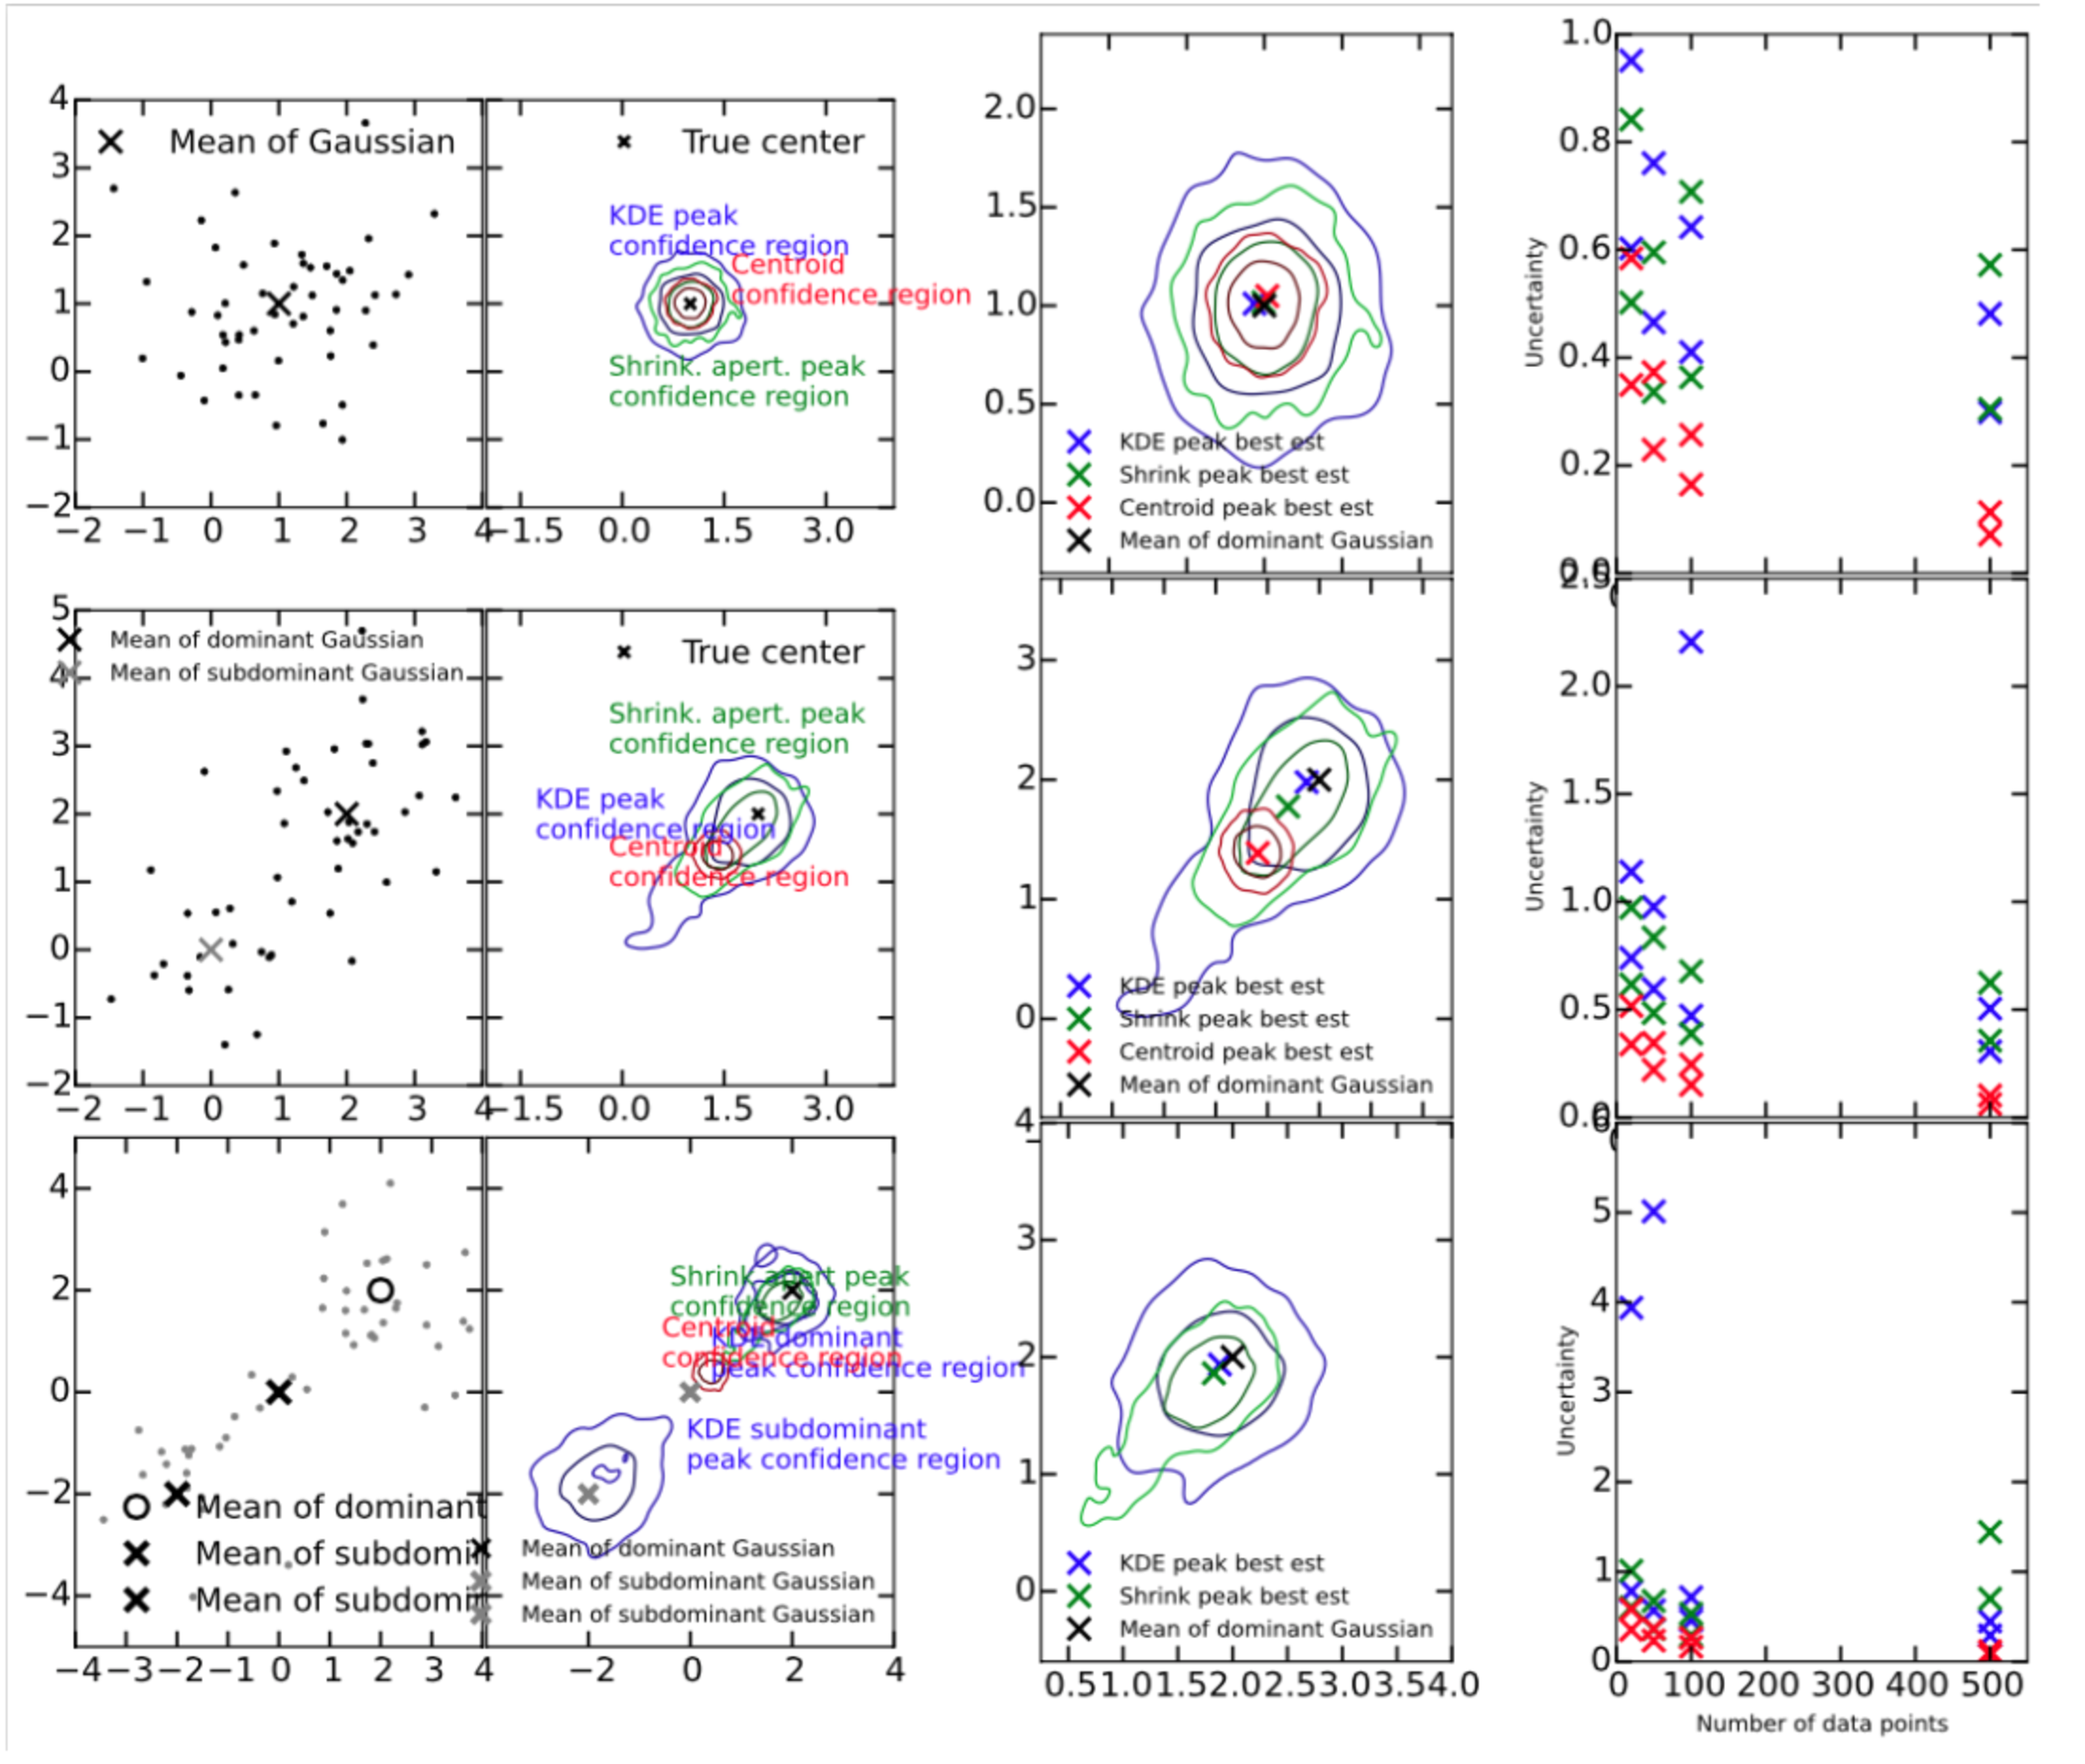
\includegraphics[width=.95\linewidth]{figures/ph_fig_galaxycenter_mixtureTests.pdf}
	\caption{}
		% \label{fig:config}}
\end{figure*}



\subsection{Comparison of the methods from test data}
In order to examine the performance of commonly used point-estimates of the
distribution of the galaxy data, we test them on data drawn from Gaussian mixtures with
known mean and variance. \\
Fig 1. one Normal mixture \\  
Fig 2. one big normal mixture and one smaller normal mixture \\ 
Fig 3. three bridged normal mixtures \\  
We compare the properties and performance of each of the
methods for finding the peaks of the galaxy and dark matter, 
except the BCG since it does not rely on the cluster member population. 
The main factors that affect the performance of the methods depend heavily on
statistical fluctuations of the drawn data. Namely, the performance of each
method depends on: 1) the
number of Gaussian mixture used, 2) the number of data points in each mixture

Due to the statistical nature of the data, it is not enough to just
compare the performance from applying each method for one realization of the
data. We also provide the 68\% and the 95\% confidence regions from the
different methods for different Monte Carlo realizations.


The details and implementation can be found in our Bitbucket git repository.



\section{Section II: DM and the lensing kernel}
To infer the 2D projected density, We reconstructed histograms of 
Since we have much higher resolution of dark matter, the choice of bin size
have smaller impact on the results.
The 2D histogram of the dark matter is analogous to a convergence map which is
a product of a weak / strong lensing analysis. 

% - [  ] Add the equation calculating a lensing kernel due to S/N constraint 
% apropos conversation with Marusa and Austin 's 


\subsection{Finding offsets} 
We computed the projected offsets between the galaxy density peaks inferred from the
cross-validated KDE and the dark matter density peak as we have shown that this
method gives us the least biased density peak estimates. 
The viewing angles of the projections are defined by an elevation angle
$\xi$ and an azimuthal angle $\phi$. 

\begin{figure*}
	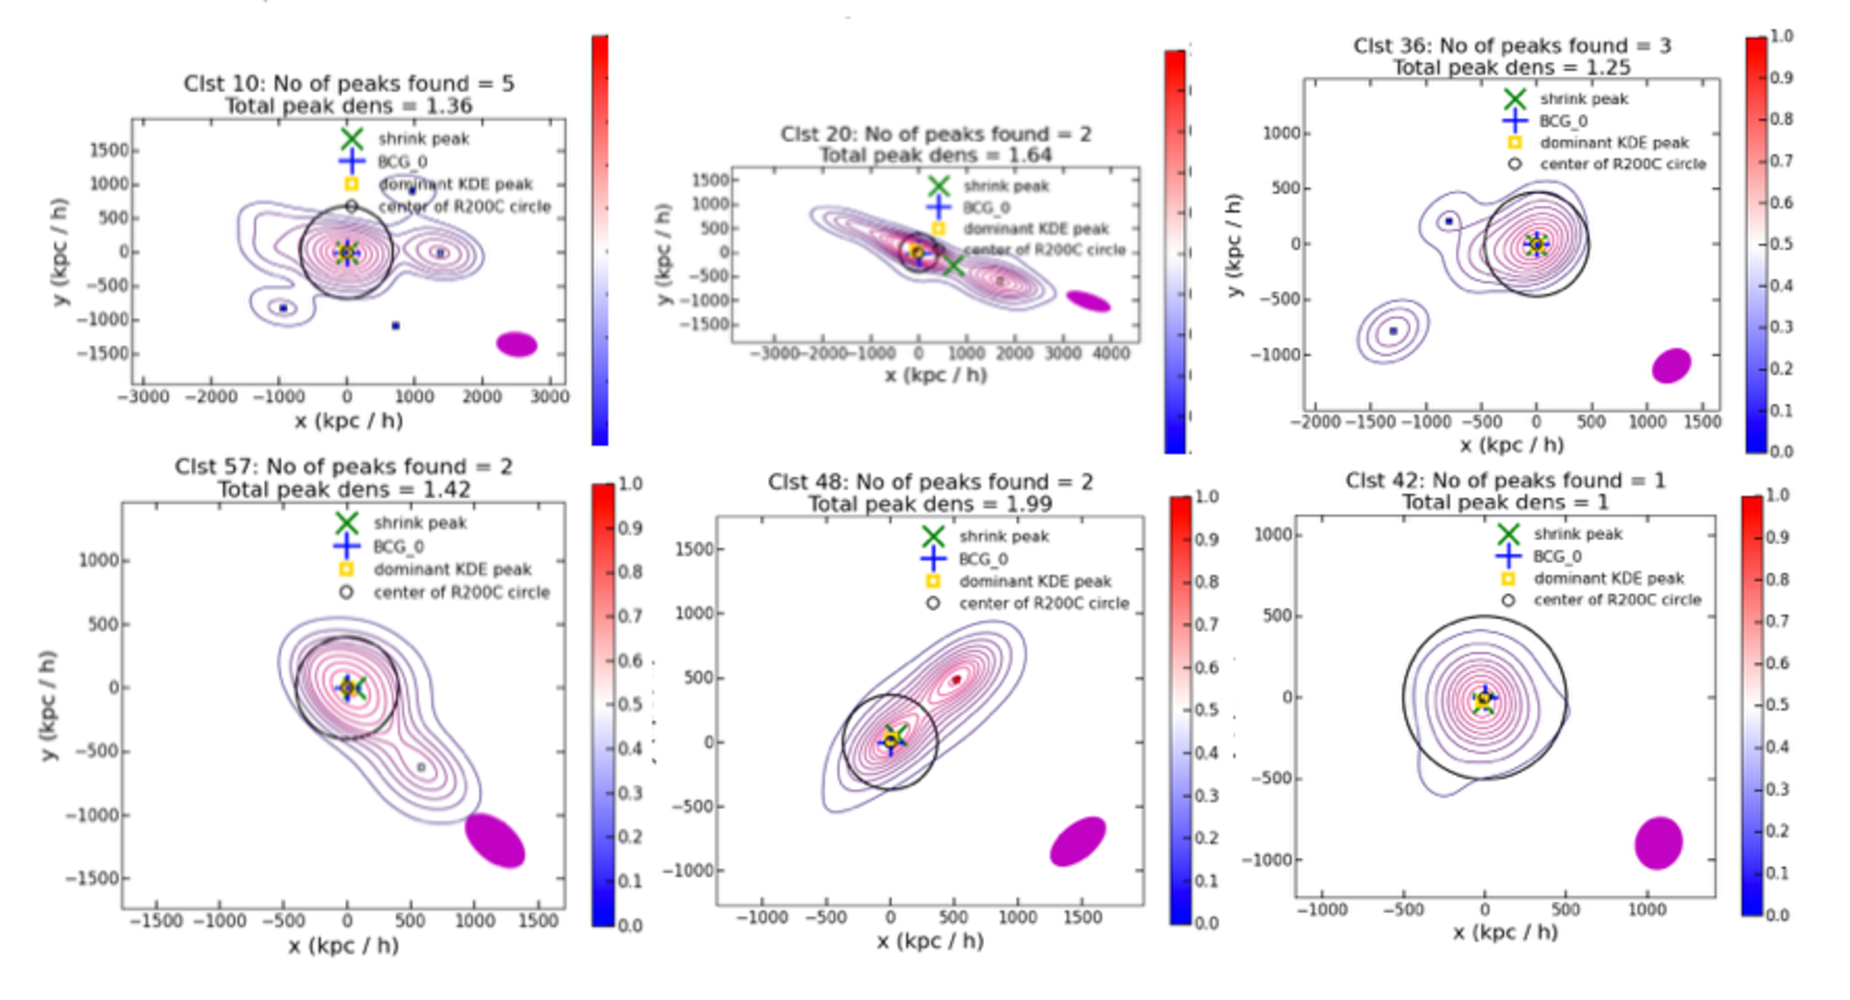
\includegraphics[width=.95\linewidth]{figures/ph_fig_galaxycenter_IllustrisClusters.pdf}
	\caption{
		\label{fig:centers}}
\end{figure*}


\begin{figure*}
	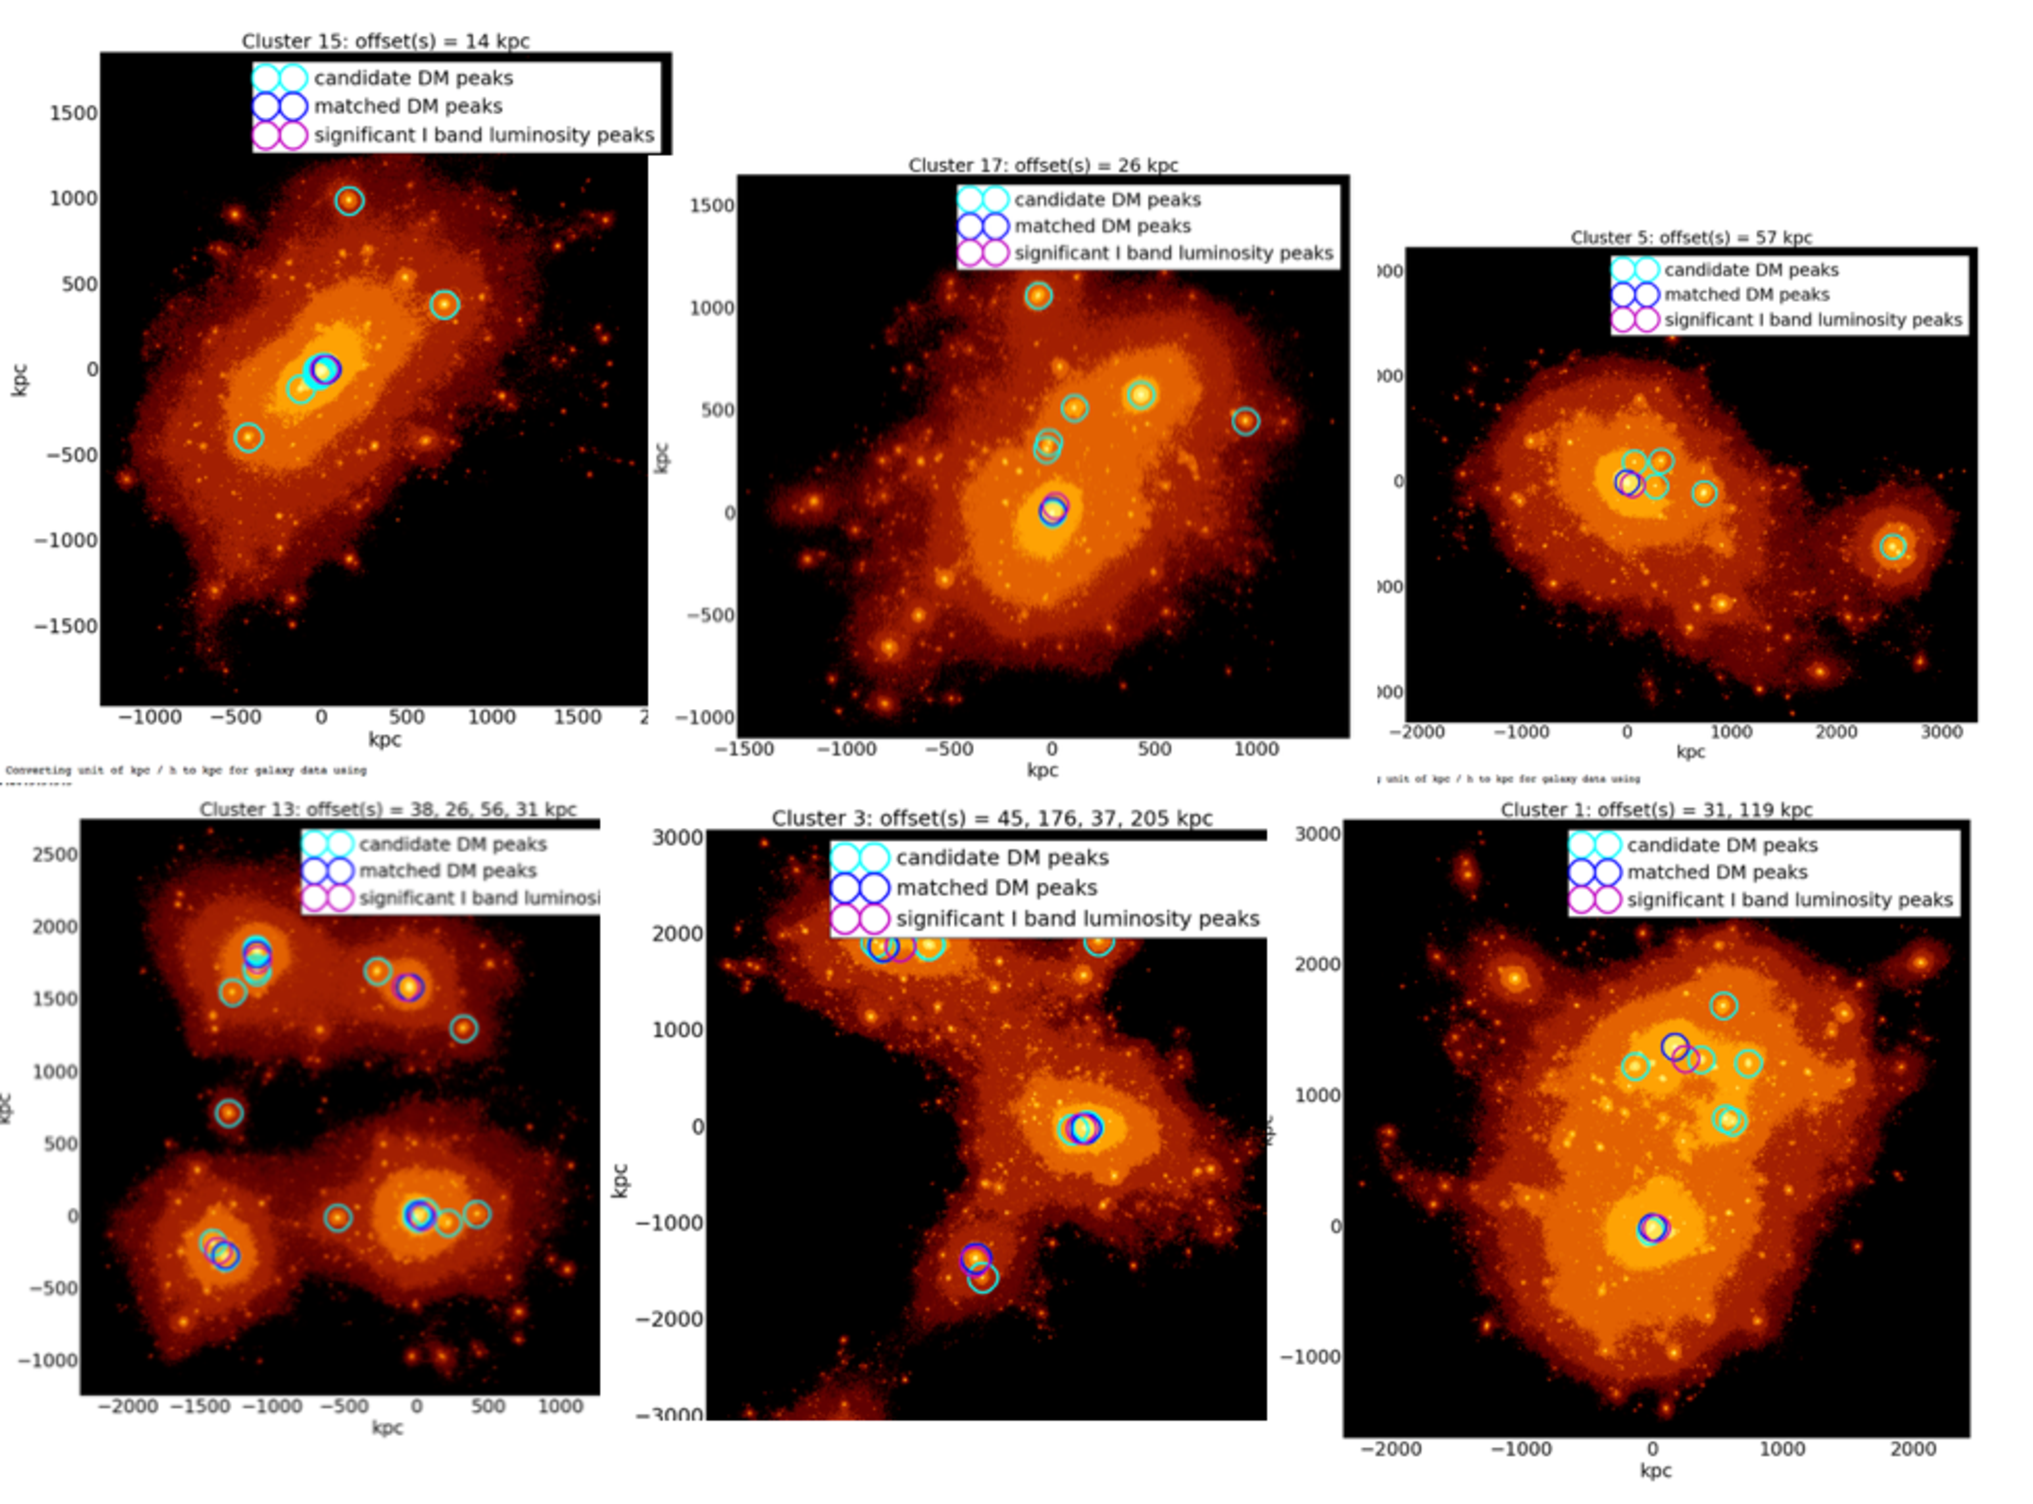
\includegraphics[width=.95\linewidth]{figures/ph_fig_DMcenter_IllustrisClusters.pdf}
	\caption{}
		% \label{fig:config}}
\end{figure*}

\section{RESULTS} 

\subsection{Galaxy-DM Offset in Illustris}
\subsubsection{Projected offsets}
* those between BCG, the most bound particle and the other masses. 


\subsubsection{Correlations between the offsets and properties of the cluster / groups}
\section{DISCUSSION}
\subsection{Comparison to other simulations}
\subsection{Comparison to other observational studies}
Central galaxy paradigm (CGP)


\subsection{Galaxy-DM Offset in Merging Galaxy Clusters}



\section{Summary}
We showed that 
\begin{itemize}
		\item  the peak finding method To-be-finalized for the density of cluster
			galaxies is the least biased due to substructures from our test data. 
		\item  all existing peak finding methods have non-negligible uncertainty 
			due to the small number of data points. When dealing with small number of
			cluster samples, the uncertainties of the peak locations should not be
			ignored.
\end{itemize}




\section{ACKNOWLEDGEMENTS}
K. Ng would like to thank Prof. D. Hogg and Prof. Thomas Lee for pointing out the ill-defined nature of
modeling galaxy clusters.
% alternative ways of characterizing differences between DM and galaxy
% distributions.

\appendix 
\section{The Physical properties of a galaxy cluster}
State variables are missing.
A galaxy cluster is not a closed system. 



\bibliographystyle{mn2e}
\bibliography{galDMoffset}
\bibliography{R_package}
\appendix
\section{KDE}
\clearpage\bsp\label{lastpage} 
\end{document}
